%%%%%%%%%%%%%%%%%%%%%%%%%%%%%%%%%%%%%%%%%%%%%%%%%%%%%%%%%%%%%%%%%%%%%%%%%%%
%
% Plantilla para un artículo en LaTeX en español.
%
%%%%%%%%%%%%%%%%%%%%%%%%%%%%%%%%%%%%%%%%%%%%%%%%%%%%%%%%%%%%%%%%%%%%%%%%%%%

\documentclass[11pt,twocolumn,spanish]{article}

% Esto es para que el LaTeX sepa que el texto está en español:
\usepackage[spanish]{babel}

% Paquetes de la AMS:
\usepackage{amsmath, amsthm, amsfonts}


\usepackage[utf8]{inputenc}
\usepackage{amsmath}
\usepackage{amsfonts}
\usepackage[spanish]{babel}
\usepackage{latexsym}
\usepackage{euscript}
\usepackage{graphicx}
\usepackage{tdclock}
\usepackage{enumerate} 
\usepackage{float}
\usepackage{multirow, array} 
\usepackage[latin1]{inputenc}
\usepackage{caption}
\usepackage[dvips]{graphicx}

% tamaño de hoja
\oddsidemargin 0.05in
\textwidth 6.3in
\topmargin -0.5in
\headheight 0in
\textheight 9in 

% Teoremas
%--------------------------------------------------------------------------
\newtheorem{thm}{Teorema}[section]
\newtheorem{cor}[thm]{Corolario}
\newtheorem{lem}[thm]{Lema}
\newtheorem{prop}[thm]{Proposición}
\theoremstyle{definition}
\newtheorem{defn}[thm]{Definición}
\theoremstyle{remark}
\newtheorem{rem}[thm]{Observación}

% Atajos.
% Se pueden definir comandos nuevos para acortar cosas que se usan
% frecuentemente. Como ejemplo, aquí se definen la R y la Z dobles que
% suelen representar a los conjuntos de números reales y enteros.
%--------------------------------------------------------------------------

\def\RR{\mathbb{R}}
\def\ZZ{\mathbb{Z}}

% De la misma forma se pueden definir comandos con argumentos. Por
% ejemplo, aquí definimos un comando para escribir el valor absoluto
% de algo más fácilmente.
%--------------------------------------------------------------------------
\newcommand{\abs}[1]{\left\vert#1\right\vert}

% Operadores.
% Los operadores nuevos deben definirse como tales para que aparezcan
% correctamente. Como ejemplo definimos en jacobiano:
%--------------------------------------------------------------------------
\DeclareMathOperator{\Jac}{Jac}

%--------------------------------------------------------------------------
\title{Caos: El orden natural}
\author{Oscar De la Cruz Echeveste\\
\small Lic. en Física  
  \small Mecánica Analítica\\
  \small Universidad de Guanajuato\\
  \small Divición de Ciencias e Ingenierias 
}

\begin{document}
\maketitle

\abstract{En el presente texto se presenta un ensayo sobre la teoría del caos. Se abordara los principales temas que se necesitan para poder caracterizar el caos en los sistemas dinámicos no lineales, Poder trabajar y determinar el carácter caótico de estos sistemas es un paso hacia adelante para poder entender la evolución en el tiempo de estos. A diferencia del carácter determinista que hasta el momento había aprendido en la carrera de física, en estos sistemas más complicados es casi imposible determinar su estado a lapsos de tiempos considerablemente grandes. Aunque esta teoría a representado un gran desafía para la ciencia, los avances que se han obtenido hasta el día de hoy nos dice que el caos es el camino al verdadero orden del universo.}

\section{Introducción}
Galileo Galilei fue matemático y astrónomo italiano del siglo XVI y XVII, conocido por muchos por su icónica riña contra los miembros de la iglesia católica al tratar de mostrarles que algunos cuerpos celeste no giraban alrededor de la tierra, como él mismo lo pudo observar en el movimiento de las lunas Jovianas. Atrevimientos como este y sumado a su carácter necio y egocéntrico lo llevaron a la excomunión y al arresto domiciliario en 1633 hasta el día de su fallecimiento en 1642 a la edad de 77 años. En el proceso en el que Galileo se adentro en la filosofía natural, observo la forma en que los cuerpos en movimiento evolucionaban a lo largo del tiempo y parecían obedecer ciertos patrones que eran predecibles al describirse de forma matemática. Tal fue su fascinación ante este hecho que dedico su vida a estudiar esta armonía que él encontraba en la naturaleza. “La matematica è la lingua in cui Dio ha scritto l'universo” es una de las frases que se le atribulen a Galileo y, aunque se desconose la veracidad de esta cita, es una frase bastante acertada. Por una extraña razón la naturaleza puede caracterizarse por modelos matemáticos con los cuales podemos predecir la evolución o cambios en el sistema con una envidiable precisión. En general, esta es la tarea a la que se adentra un físico. La matemática se vuelve la herramienta de trabajo más poderosa que da paz y tranquilidad a la certidumbre que caracteriza y predice la evolución de los sistemas. Pero la realidad es más complicada de lo que se espera. Ciertamente, la dinámica de muchos de los sistemas que se estudian no es tan sencilla de predecir. Uno se estos sistemas, y tal vez el de mayor antigüedad, es el problema de los tres cuerpos, el cual consta de tres objetos celestes en movimiento afectados por la gravedad de cada uno. Tanto Newton (1642-1727) como sus predecesores matemáticos han estudiado este problema por los últimos siglos. Fue el matemático francés Henri Poincaré (1854 - 1912) quien demostró que no había una solución analítica para este problema y agrego que esto representaba la naturaleza del caos. 

Poincaré fue un pionero en el estudio del caos, un concepto que hasta hoy en día parece ser desconocido para muchos, temido por algunos y apasionado para otros pero sin duda un dolor de cabeza para todo aquel estudioso de esta área. Trabajar con el caos significa trabaja con sistemas dinámicos no lineales y la ecuación que los caracteriza es de la forma:
\begin{equation}
\frac{dx}{dt} = f(x,t;\alpha)  \quad \cite{sd}
\end{equation}
Que muesta como el sistema cambia su estado en el tiempo basado en sus condiciones iniciales y paramtros como $\alpha$ y siendo la función $f(x,t;\alpha)$ de forma no lineal.

Los sistemas dinámicos pueden ser discretos y continuos. Los sistemas discretos toman el paso del tiempo como cantidades de números enteros, por ejemplo la ecuación $x_{n+1} = mx_{n}(1-x_{n})$ muestra como evoluciona $x$ conforme el tiempo, en este caso  $n$, avanza en una unidad. En cambio, los sistemas dinámicos discretos se expresan como ecuaciones diferenciales $\frac{dx}{dt} = mx(1-x)$ donde, de nuevo $x$ cambia en el tiempo pero de forma infinitesimal. Ademas de esto, como ya se menciono, para sistemas que conllevan al caos, las ecuaciones que describe el sistema son no lineales y son más complejos de analizar. El comportamiento de estos sistemas parece impredecible y la armonía con la que solía describir la evolución de un sistema en el tiempo como lo veían grandes personajes como Galileo Galilei peces venirse cuesta abajo y el determinismo al que tanto estamos acostumbrado los estudiantes de la física ya no toma lugar en las hojas de su estudio. El matemático británico James Lighthill (1924-1998) en el año de 1966 declaro a la sazón presidente de la Unión Interna de Mecánica Pura y Aplicada lo siguiente:

“Llegados a este punto debo hacer un alto y hablar en nombre de la gran hermandad de los expertos de la mecánica. Hoy somos muy consientes de que el entusiasmo que sentían nuestros predecesores por el éxito maravilloso de la mecánica newtoniana les llevó a hacer generalizaciones, en el campo de la predicción …, que hoy han resultado ser falsas. Queremos pedir disculpas colectivamente por haber inducido a error al público culto al propagar, a propósito del determinismo de los sistemas que cumplen las leyes de newtonianas del movimiento, unas ideas que sesgues de 1960 ya no se pueden sostener.” \cite{lig} 

Ilya Prigogine menciona esta cita en su libro las leyes del caos para deshacerse de la idea determinista que había tomado la mecánica hasta esos días y menciona: “Durante mucho tiempo el determinismo era el símbolo de la inteligibilidad científica, mientras que hoy se reduce a una propiedad que sólo es válida en casos límites (sistemas dinámicos estables)”\cite{ilya1}.


\section{Mapeo}\label{sec:nada}
En matemáticas un mapeo, aplicación o  función es una regla que asocia valores de algún conjunto que llamaremos \textit{conjunto objeto} \textbf{A} a un \textit{conjunto objetivo} \textbf{B}. Podemos representar esto de manera gráfica como:

\begin{equation*}
\begin{split}
&f:  A \longrightarrow B \\
&a  \mapsto f(a) = b  
\end{split}
\end{equation}

Donde $f$ es la regla de asociación entre los valores del conjunto A (en este caso a)  a los valores del conjunto B (en este caso b). Un ejemplo sencillo es una función $f:  \mathbb{R} \longrightarrow \mathbb{R} $ tal que $x \mapsto f(x) = 2x$ donde la función $f$ relacionas los elementos del conjunto de los números reales con los elementos de un conjunto igual de tal forma que cada elemento del conjunto objetivo es el doble de un sólo elemento del conjunto objeto. En la \textbf{ figura 2.1} se puede ver un ejemplo gráfico de un mapeo entre un conjunto de todas las pelotas deportivas y los números naturales $\mathbb{N}$. Este mapeo podría ser una regla como: “las pelotas de un sólo color tendrán el valor de uno, las pelotas de un dos colores tendrán el valor de dos, las pelotas de tres colores tendrán el valor de tres, … ”. 

\begin{figure}[H]
\centering
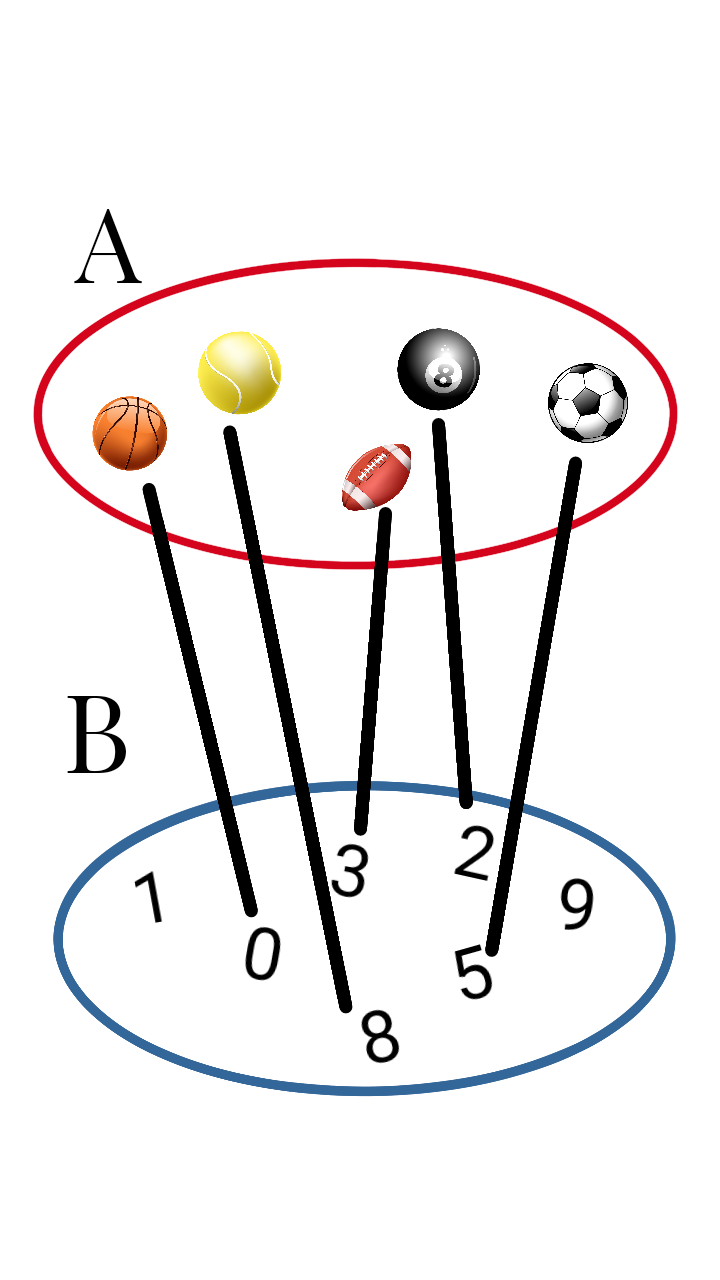
\includegraphics[width=3cm]{figura_1}
\caption*{\textbf{Figura 2.1}: Representación gráfica de un mapeo de conjuntos del pelotas deportivas al conjunto de números naturales $\mathbb{N}$ }
\label{etiqueta}
\end{figure}
\end{enumerate}

En teoría de sistemas dinámicos los mapeos son usados para crear sistemas dinámicos discretos y así poder caracterizar su evolución. Esto se consigue usando mapeos iterativos los cuales se construyen en base a una función:

\begin{equation}
x_{n+1} = f(x_{n})
\end{equation}

Es decir, una función que depende de $x_n$  determinara el valor que tomara $x_{n+1}$ a travez de la aplicación $f$ y este a su vez al evaluarse $f(x_{n+1})$ determinara el siguiente valor $x_{n+2}$.  Un ejemplo común para entender este proceso es el  \textbf{mapeo logístico}. Este proviene de modelar el crecimiento para una población biológica y tiene la siguiente forma:

\begin{equation}\label{eq:log}
x_{n+1} = f_{A}(x_{n}) = Ax_{n} (1-x_{n})
\end{equation}

Para su construcción tomaremos el ejemplo de Robert C. Hilborn de su libro “Chaos and Nonlinear Dynamics: an introduction for scientists and engineers” \cite{Cd94} y lo haremos de la misma forma. Analizando la población de mariposas que nacen y mueren a lo largo de un año podemos saber que la cantidad de mariposas $N_{1}$ al terminar el año depende de la cantidad de estas que había al comenzar $N_{0}$ y ademas considerando del entorno en el que viven. Este ultimo factor se incluye como un número $A$ de tal forma que si $A>1$ el número de mariposas crece y lo contrario si $A<1$ . De tal forma que tenemos la siguiente relación:

\begin{equation*}
N_{1} = A N_{0}
\end{equation}  

Ahora, considerando que al incrementar demasiado la población al final no habrá suficiente comida para toda la población y causará una muerte masiva de mariposas. Así, el crecimiento de la población se ve limitado por éste factor por lo que es necesario agregar un termino con esta información. Escogemos un factor proporcional a $N^2$ para que su influencia sea poca para $N's$ pequeñas pero volviendoce más importante para $N's$ más grandes:

\begin{equation*}
N_1 = AN_0 - BN_0^2
\end{equation}
En general:
\begin{equation}\label{eq:Ns}
N_{n+1} = AN_n - BN_n^2
\end{equation}

De esta forma el segundo termino hará que decresca la población. De la ecuación (\ref{eq:Ns}) podemos ver que hay un valor maximo de población. Cuando $N_n = \frac{A}{B}$ entonces $N_{n+1} = 0$ por lo tanto la población esta muerta. Entonces, tenemos un valor máximo para $N$:
\begin{equation}
N^{max} = \frac{A}{B}
\end{equation}

Así, podemos definir una nueva variable $x_n$ que presenta la población como una frección de la máxima poblacion posible
\begin{equation}
x_n = \frac{N_n}{N^{max}}
\end{equation} 
Así llegamos a la expreción (\ref{eq:log}):
\begin{equation*}
x_{n+1} = Ax_{n} (1-x_{n})
\end{equation}
Donde $x$ adquiere valores sólo entre 0 y 1, representando la población en $n$ número de años. Por ejemplo, si inicialmente tenemos una población de $x_0 = 0.2$ con un factor de entorno $A = 0.5$, entonces, la población en un año será $x_1 = 0.5*0.2*(1-0.2) = 0.08$ y para el siguiente año será $x_2 = 0.5*0.08*(1-0.08) = 0.0368$. Si seguimos iterando para un pasar de años mayor se llegará a que $x=0$, es decir, la pabración se extinguirá. En la \textbf{figura 2.2} vemos la evolución de cinco poblaciones con tres A's distintas y $x$'s iniciales  $0.1,0.2,0.3,0.4,0.5$. 

\begin{figure}[H]
\centering
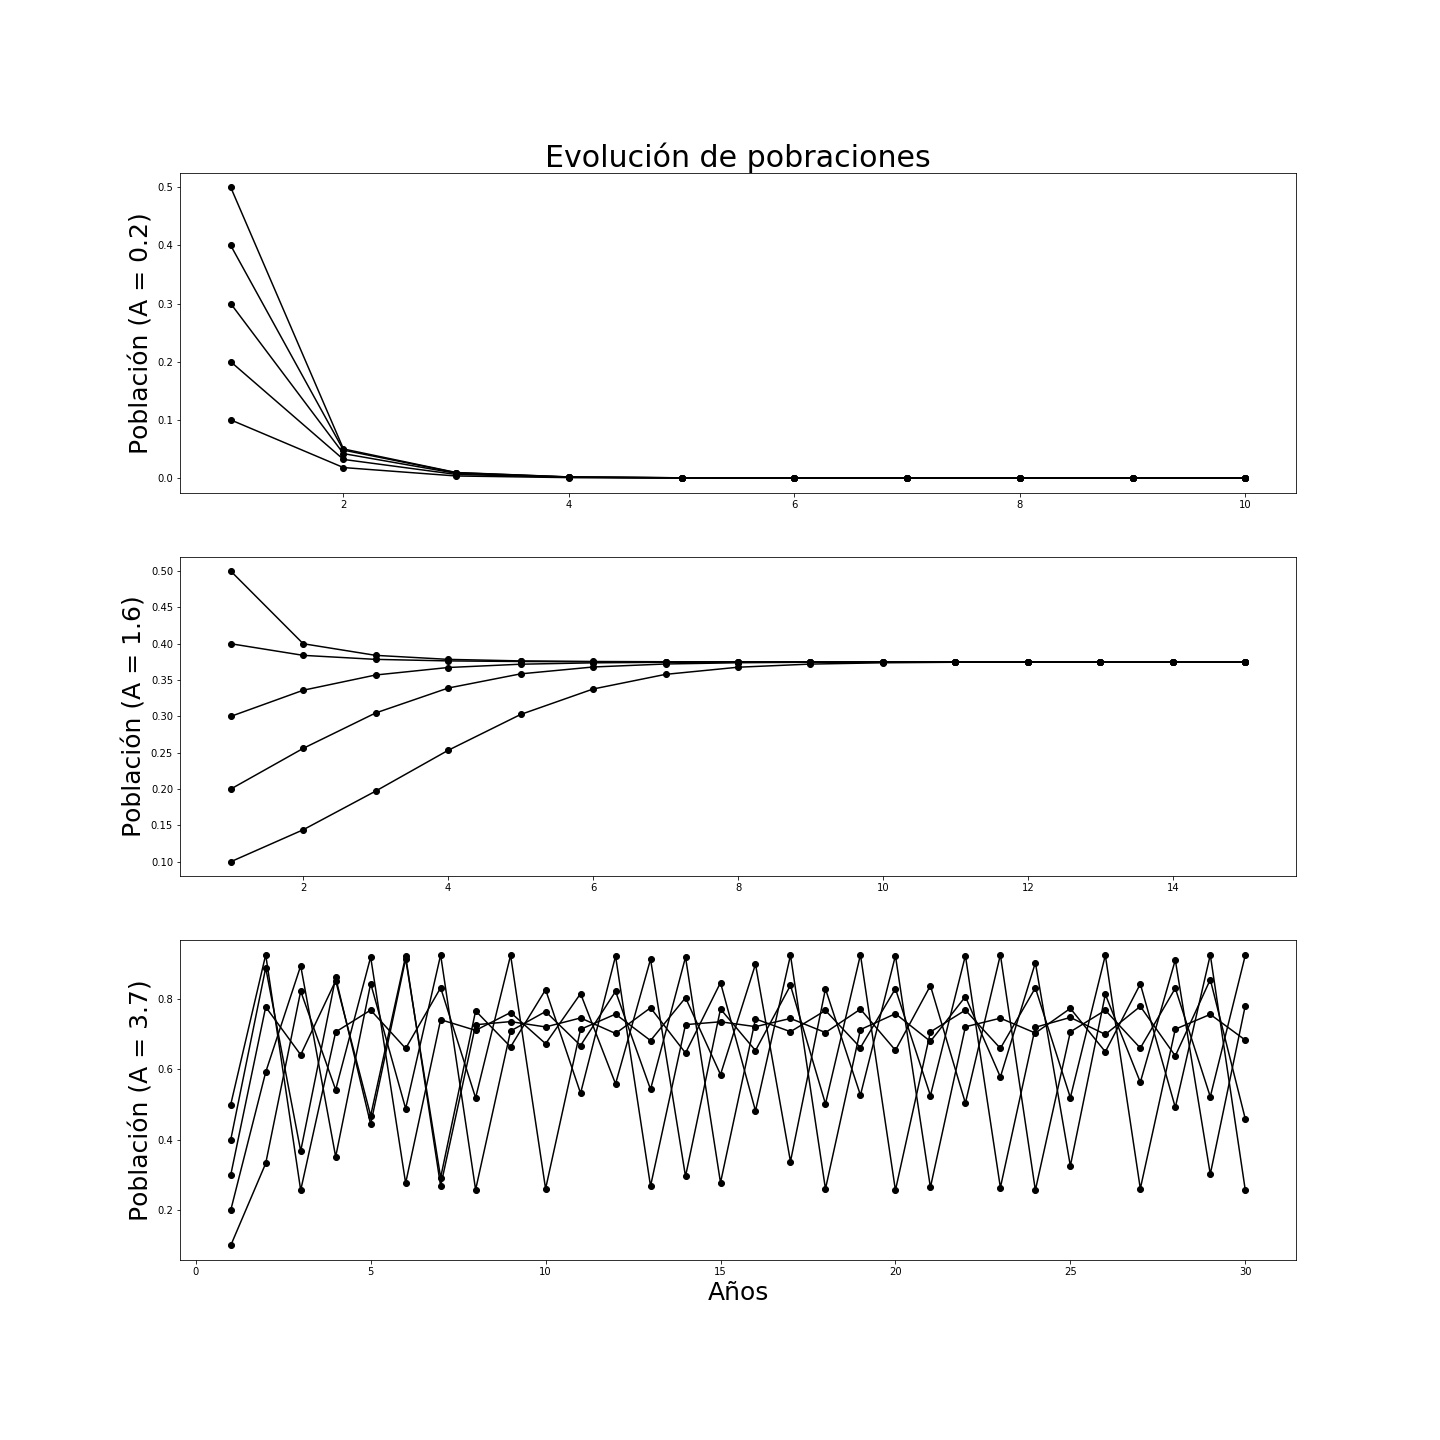
\includegraphics[width=7cm]{logistico.jpg}
\caption*{\textbf{Figura 2.2}: Evolución de 5 poblaciones con $x$ iniciales de $0.1,0.2,0.3,0.4,0.5$ y A's $0.2,1.6,3.3$.}
\end{figure}

En la primera figura vemos como todas las poblaciones se extinguen en un al paso de cierto número de años. En la segunda las poblaciones convegen a un número espesifico de poblacion. La ultima figura muestra como la evolución de las poblaciones para  $A=3.7$ no converge a un número espesífico, sino que toma valores que parecen arbitrarios. Ahora, en la \textbf{figura 2.3} se muestra el diagrama de bifurcación del mapeo logístico. Se grafica el valor que toma $x$ al pasar cieta cantidad de años (cantidad de iteraciones) contra los valores de $A$ que van de dos a cuatro.

\begin{figure}[H]
\centering
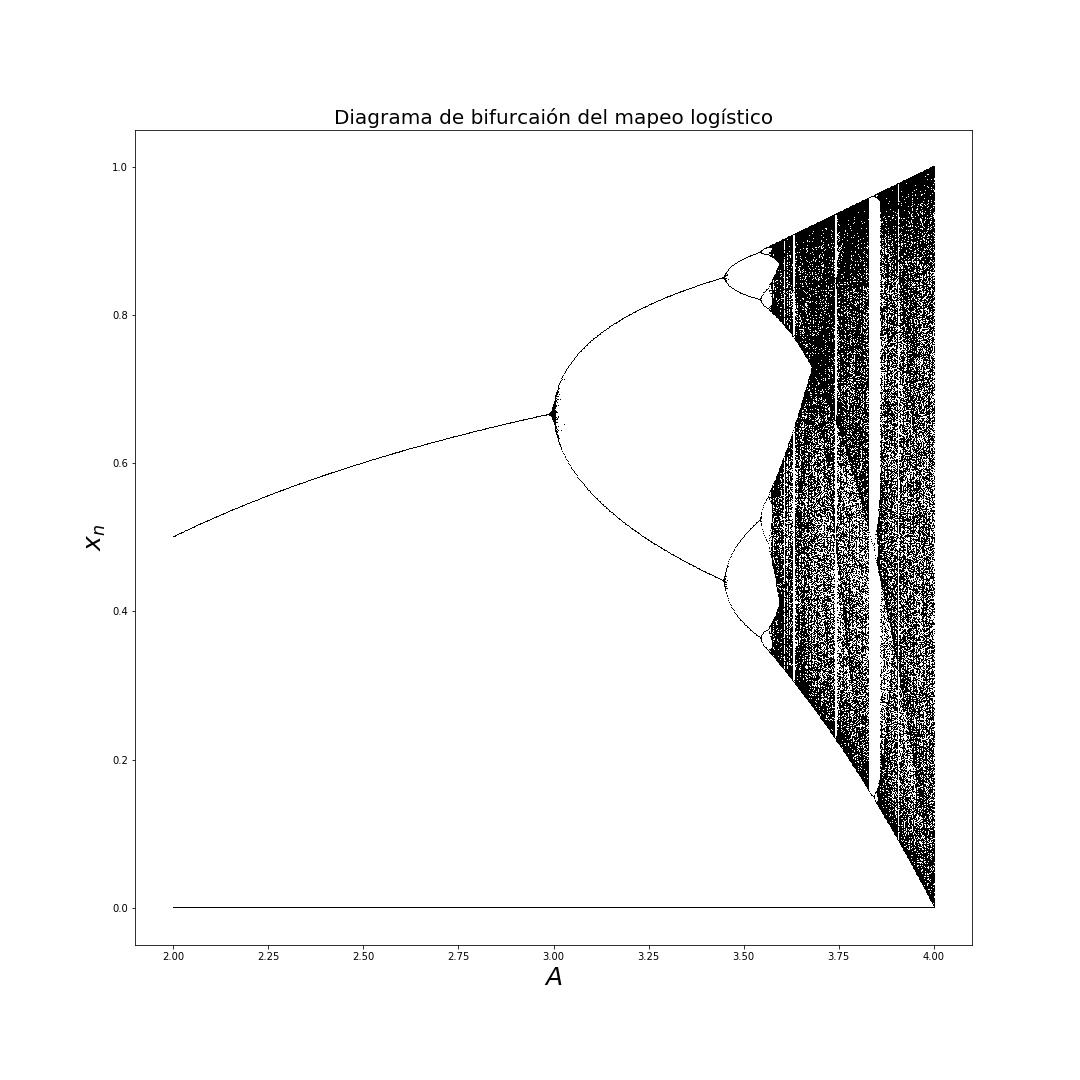
\includegraphics[width=7.5cm]{map_log}
\caption*{\textbf{Figura 2.3}: Diagrama de bifurcación del mapeo logístico.}
\label{etiqueta}
\end{figure}


Se puede apreciar que para $A>3$ los valores a los que puede llegar el número de población $x$ cada ves son mayores. En especial, para $A>3.5$ los valores de que puede tomar $x$ parecen totalmente arbitrarios. Aquí tenemos un buen ejemplo del caos. Para un parametro $A>3.5$ para condiciones iniciales $x$ que difieren un poco, el valor de la población final puede ser totalmente diferente.

\section{Atractores Extraños}

Los sistemas dinámicos son en general sistema disipativo que esta sujeto a una fuerza externa que, de no ser por esta, el sistema se detendría en un determinado  tiempo. Por consecuencia de estas fuerzas externas los sistemas tienden a evolucionar a una trayectoria específica independiente las condiciones iniciales. A estos conjuntos de estados a los que converge un sistema dinámico se les llama \textit{atractor}. Un ejemplo sencillo es un oscilador armónico forzado. Este sistema comienza en una cierta posición y velocidad (que son las condiciones iniciales), el sistema, al ser disipativo por la fricción que hay con su entorno, pierde energía tiende a llegar al reposo, pero debido a una fuerza estrena que se le aplica mientras esta en movimiento se comenzara a contrarrestar la fuerza de fricción y llegara el momento en que la energía disipada será igual a la inyectada al sistema por lo que su movimiento convergerá a una trayectoria que caracteriza a un oscilador armónico sin amortiguamiento ni fuerza externa. En la \textbf{figura 3.1} se muestra el espacio fase de un oscilador armónico forzado $\ddot\theta + \mu \dot\theta + \omega_0^2 sin(\theta) = A\cos(\omega_d t)$ donde se ve su evolución hasta converger a una trayectoria ovalada.

\begin{figure}[H]
\centering
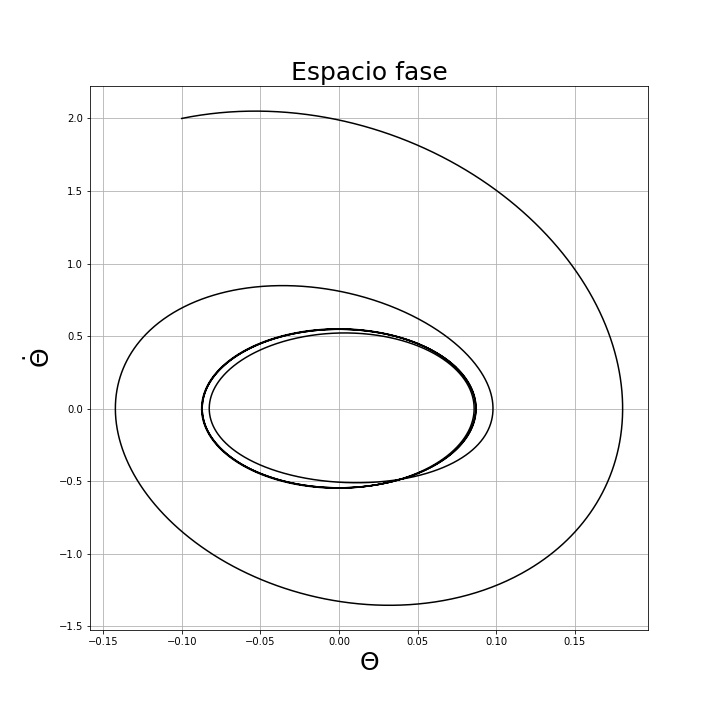
\includegraphics[width=7cm]{pendulo.jpg}
\caption*{\textbf{Figura 3.1} espacio fase de un oscilador armónico forzado $\ddot\theta + \mu \dot\theta + \omega_0^2 sin(\theta) = A\cos(\omega_d t)$ con condiciones iniciales, $\theta(t=0) = -0.1$, $\dot\theta(t=0) = 2$ y parametros $\mu = \frac{3\pi}{2}$, $\omega_0 = 3\pi$ y $\omega_d  = 2\pi$ }
\label{etiqueta}
\end{figure}
\end{enumerate}

Un atractor puede presentarse como un punto o como una trayectoria específica en el espacio fase del sistema dinámico. En un sistema caótico la trayectoria a la que converge la solución tiene la forma de un fractal (En la sección de fractales se hablara más de este concepto) debido a la dinamica caotica del sistema y se les llama \textbf{atractores extraños}. En estos casos, una vez que el sistema se encuentra en el atractor, los estados cercanos divergen entre sí. Es decir, el sistema nunca vuelvera al mismo lugar, pero despues de cierto tiempo el sistma puede estar muy cercano a los estados ateriores. 

El atractor más famoso en teoría de caos es el atractor de Lorenz. En el año 1963, el profesor Edward Lorenz(1917-2008), matemático y meteorólogo, al tratar de desarrollar un modelo matemático simple para describir la dinámica de convección atmosférica llego las siguientes tres ecuaciones:
\begin{equation} 
\begin{split} 
\frac{dx}{dt} & = a(y-x) \\
\frac{dy}{dt} & = x(b-z) - y\\
\frac{dz}{dt} & = xy-cz 
\end{split} 
\end{equation} 
Las ecuaciones describen la dinámica de un fluido con una diferencia de temperatura entre la parte superior e inferior de éste. Donde la variable $x$ es proporcional a la velocidad de convección y a su vez $y$ y $z$ son proporcionales a la variación de temperatura horizontal y vertical respectivamente. \textbf{La figura 3.2} muestra la solución de forma gráfica al sistema de ecuaciones y puede observarse el conjunto continuo de estados a los que converge el sistema. 
\begin{figure}[H]
\centering
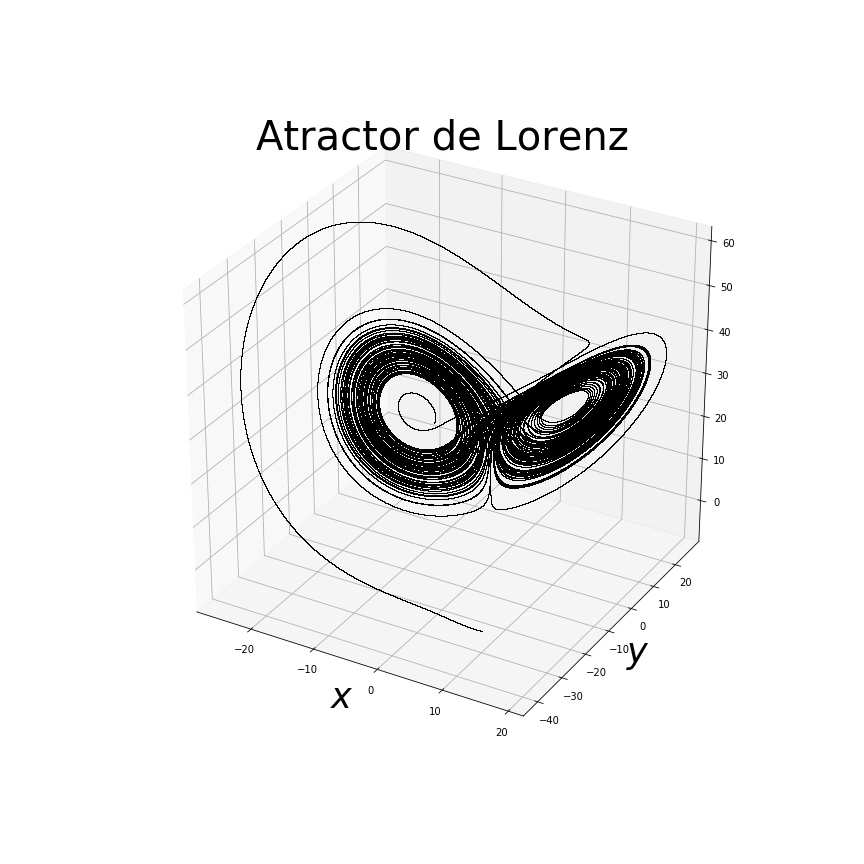
\includegraphics[width=7cm]{atrac_lor.jpg}
\caption*{\textbf{Figura 3.2} Atractor de Lorenz con parametros $a=10$, $b=28$, $c=8/3$ \cite{AL} y condiciones iniciales $x_0=10$, $y_0=-30$, $z_0=-5$ }
\label{etiqueta}
\end{figure}
\end{enumerate}
\section{Secciones de Poincaré}
Al estudiar los sistemas dinámicos es muy probable que se encuentren soluciones con trayectorias bastante complicadas de determinar. Para simplificar el análisis de la solución, se opta por buscar una representación de las solución sin mayor detalle a diferencia del que se muestra en el espacio fase. Las secciones de Poincaré son una herramienta útil para llevar a cabo esta tarea por medio de intersecciones perpendiculares de hiperplanos en la trayectoria que muestra la evolución del sistema. Las secciones se pueden construir de forma sencilla. Tenemos un sistema dinámico:
\begin{equation}
\frac{dx}{dt} = f(x,t;\alpha) 
\end{equation}
Cuya solución describe una órbita periódica, que llamaremos $\Lambda$, en un punto $x_0$ donde se construye un plano perpendicular a este. Así, para cualquier punto $x$ próximo a $x_0$ en el mismo plano perpendicular, la solución del sistema dinámico que pasa por $x$ en $t=0$, atravesará de nuevo el plano en el punto $P(x)$ próximo a $x_0$. Tenemos entonces el mapeo
\begin{equation}
\begin{split}
&P:  U \longrightarrow S \\
&x_{n} \mapsto x_{n+1} = P(x_{n})  
\end{split}
\end{equation} 
Donde U es una vecindad del punto $x$ en el plano S \cite{sd}. A esto se le llama el mapeo, sección o aplicación de Poincaré que es presentada en 1881 por Henri Poincaré. En la \textbf{figura 4.1} se puede ver de forma gráfica la construcción del plano en una trayectoria en tres dimenciones (atractor de Lorenz).

\begin{figure}[H]
\centering
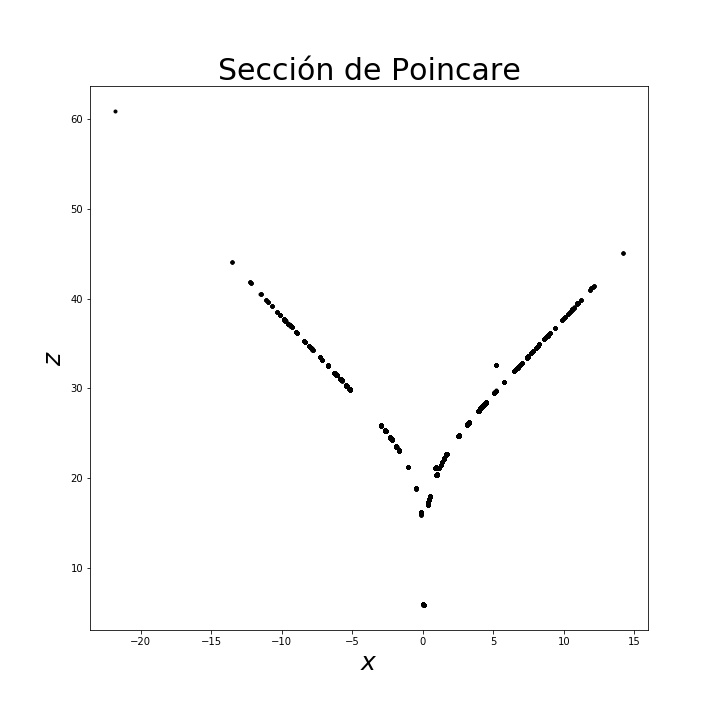
\includegraphics[width=7cm]{sec_poin.jpg}
\caption*{\textbf{Figura 4.1}: Sección de Poincare  }
\label{etiqueta}
\end{figure}
\end{enumerate}

En la mayoría de casos, el mapeo de Poincaré se reduce a un mapeo iterativo unidimensional. Sin embargo, hay soluciones de sistemas que requieren de mayor información.

\section{Exponente de Lyapunov}
Como hemos visto, en un sistema dinámico no lineales encontrar las soluciones que caracterizan la evolución de sistema a lo largo del tiempo se vuelve muy complicado. Ademas, estos sistemas tienden a ser muy sensibles a las condiciones iniciales, es decir, una diferencia mínima en la configuración en el que el sistema comienza, representara una amplificación exponencial. Unas causas tan pequeñas como se quiera tienen consecuencias esenciales en el comportamiento del sistema. La separación entre dos trayectorias cercanas aumenta exponencialmente con el tiempo $s(t) = s(t=0) e^{\lambda t}$ siendo $s = (\delta x)_t$ y  $s(t=0) =  (\delta x)_0$ \cite{ilya2}. Donde $\lambda$ los llamados coeficientes de Lyapunov y de esta forma, los sistemas que presentan esta divergencia, se les asocia un comportamiento caótico.

Para contar la herramienta matemática que nos de la información sobre la separación de las trayectorias en un sistema dinámico, tenemos que medir la distancia que hay entre estas.Dado un sistema dinámico de la forma $\frac{dx}{dt} = f(x)$ la velocidad de cambio de separación entre 2 trayectorias \cite{172}:
\begin{equation*}
\begin{split}
\frac{ds}{dt} &= \frac{dx}{dt} -\frac{dx_0}{dt}\\
&=f(x) - f(x_0)\\
\end{split}
\end{equation}
Asumiendo que $x$ esta cercano a $x_0$ usamos la expansión en serie de de Taylor:
\begin{equation*}
f(x) = f(x_0) + \frac{dx}{dt}|_{x_0} (x-x_0)
\end{equation}
Y por tanto tenemos que:
\begin{equation}
\frac{ds}{dt} = \frac{dx}{dt}|_{x_0} (x-x_0)
\end{equation} 
Al esperar que la distancia cambie exponencialmente obtenemos:
\begin{equation}
\begin{split}
s(t) &= s(t=0) e^{\lambda t }\\ 
\frac{ds}{dt} &= \lambda s(t=0)e^{\lambda t} = \lambda s
\end{split}
\end{equation} 
Donde podemos ver que:
\begin{equation}
\lambda = \frac{dx}{dt}|_{x_0} (x-x_0)
\end{equation} 

De esta forma, podemos encontrar el coeficiente $\lambda$ que acompañan al exponente de Lyapunov. Si $\lambda<0$ es fácil ver que la distancia $s$ converge por la potencia negativa del exponencial y si  $\lambda>0$ $s$ diverge. Por lo tanto, los sistemas caóticos son aquellos que tienen coeficientes de Lyapunov positivos. Así podemos obtener la información del carácter estable o caótico de los sistemas dinámicos. 

Ahora, para calcular los exponenetes de Lyapunov sobre una série de datos y asi obtener los coeficientes de el mapeo logístico de la sección mapeos.

Al tener una série de datos $x_0, x_1,x_2,...$ tal que $x_i = x(t_i)$. Asumimos que el tiempor entre dos posiciones $x$ cotinuas es siempre igua, por tanto:
\begin{equation}
t_{n} - t_0 = n\tau
\end{equation}  
La distancia entre cada ponto continuo será:
\begin{equation}
\begin{split}
s_0 &= |x_j - x_i|\\
s_1 &= |x_ {j+1} - x_{i+1}|\\
s_2 &= |x_ {j+2} - x_{i+2}|\\
&.\\
&.\\
s_n &= |x_ {j+n} - x_{i+n}|\\ 
\end{split}
\end{equation}  

Asumimos que estos valores incrementan exponencialmente con un incremento en el tiempo de n, tendremos:
\begin{equation}
s_n = s_0 e^{\lambda n}
\end{equation} 
Por lo tando, 
\begin{equation}
\lambda = \frac{1}{n} \ln \frac{s_n}{s_0}
\end{equation}  

Y para obtener el promedio de los coeficiente de Lyapunov para N cantidad de datos:

\begin{equation}
\lambda = \frac{1}{N} \sum_{i = 1}^N \lambda(x_i)
\end{equation}

Dodne $\lambda(x_i)$ se puede obtener por derivación (ecuación 12). La \textbf{figura 3.2} muestra la gráfica de coeficioentes de Lyapunov $\lambda$ conta el el coeficiente  $A$ del mapeo logístico. 

\begin{figure}[H]
\centering
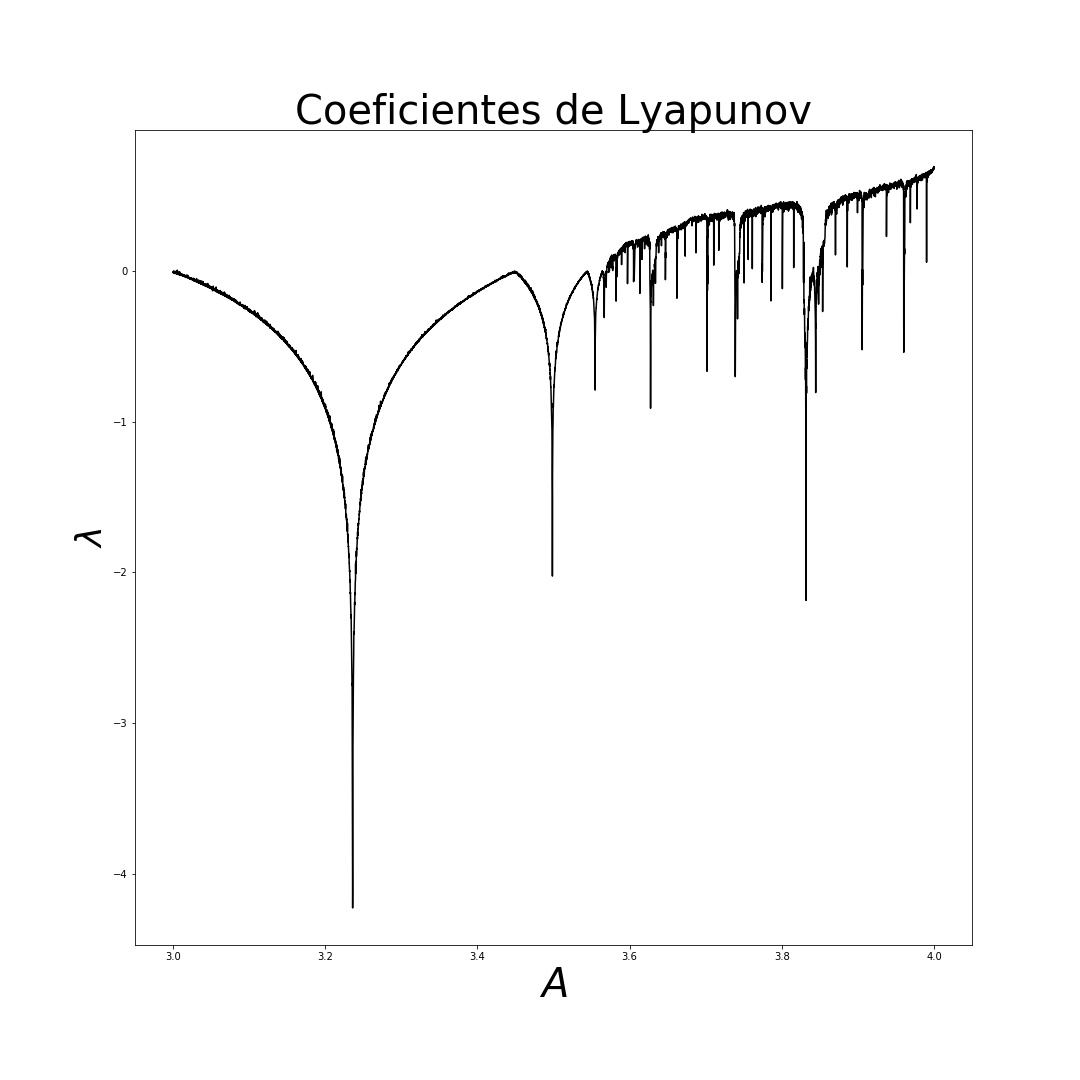
\includegraphics[width=7cm]{lyapunov.jpg}
\caption*{\textbf{Figura 3.2} Coeficientes de Lyapuniv}
\label{etiqueta}
\end{figure}
\end{enumerate}

La gráfica muesta como las regiones de ausencia de caos para los valores de $A$, es decir, donde $\lambda<0$ y los valores donde se presenta el comportamiento caótico con $\lambda>0}$.

\section{Fractales}

“ ¿Por qué a menudo se describe la geometría como algo frío y seco?. Una de las razones es su incapacidad de describir la forma de una nube, una montaña una costa o un árbol.”\cite{frac}

Los fractures son figuras geométricas que resultan muy atractivas, podría decir que es unas de las pocas cosas que tienen la matemática que a todo el mundo le gusta. La forma que toman estas figuras son por medio de patrones repetitivos y que a escalas arbitrarias la figura tiene las misma forma. En otras palabras, un fractal se dibuja haciendo patrones que al acercarte o alejarte de la figura se seguirá viendo el mismo patrón. Dibujar estas figuras en la realidad resulta imposible ya que su carácter a escalas infinitamente pequeñas o grandes sólo es concebible de forma abstracta. Un ejemplo sencillo, que se puede hacer manualmente acercadoce a la forma de fractal, es un triángulo como se muestra en la figura 6.1. Se comenza dibujando un triangulo equilátero para después dividirlo en cuatro secciones triangulares iguales y en cada triángulo de las esquinas se hace exactamente lo mismo, dividir en  secciones triangulares y hacerlo otra vez en cada esquina. Así tenemos una figura llamada el \textit{triángulos de Sierpinski Gasket} que al acercarte, por ejemplo a la punta del triangulo principal, se verá el mismo patrón de triángulos divididos en las mismas secciones. 


\begin{figure}[H]
\centering
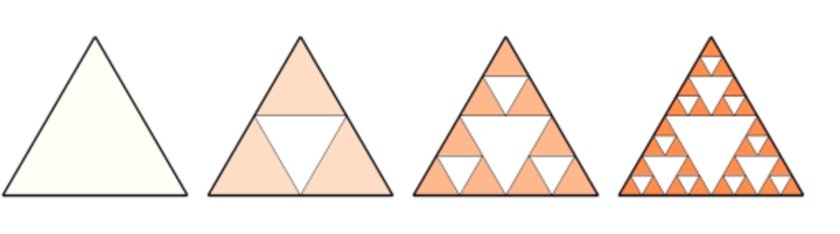
\includegraphics[width=7cm]{triangulo2.jpg}
\caption*{\textbf{Figura 6.1} Construcción del triángulos de Sierpinski Gasket \cite{triangulo}}
\label{etiqueta}
\end{figure}

\begin{figure}[H]
\centering
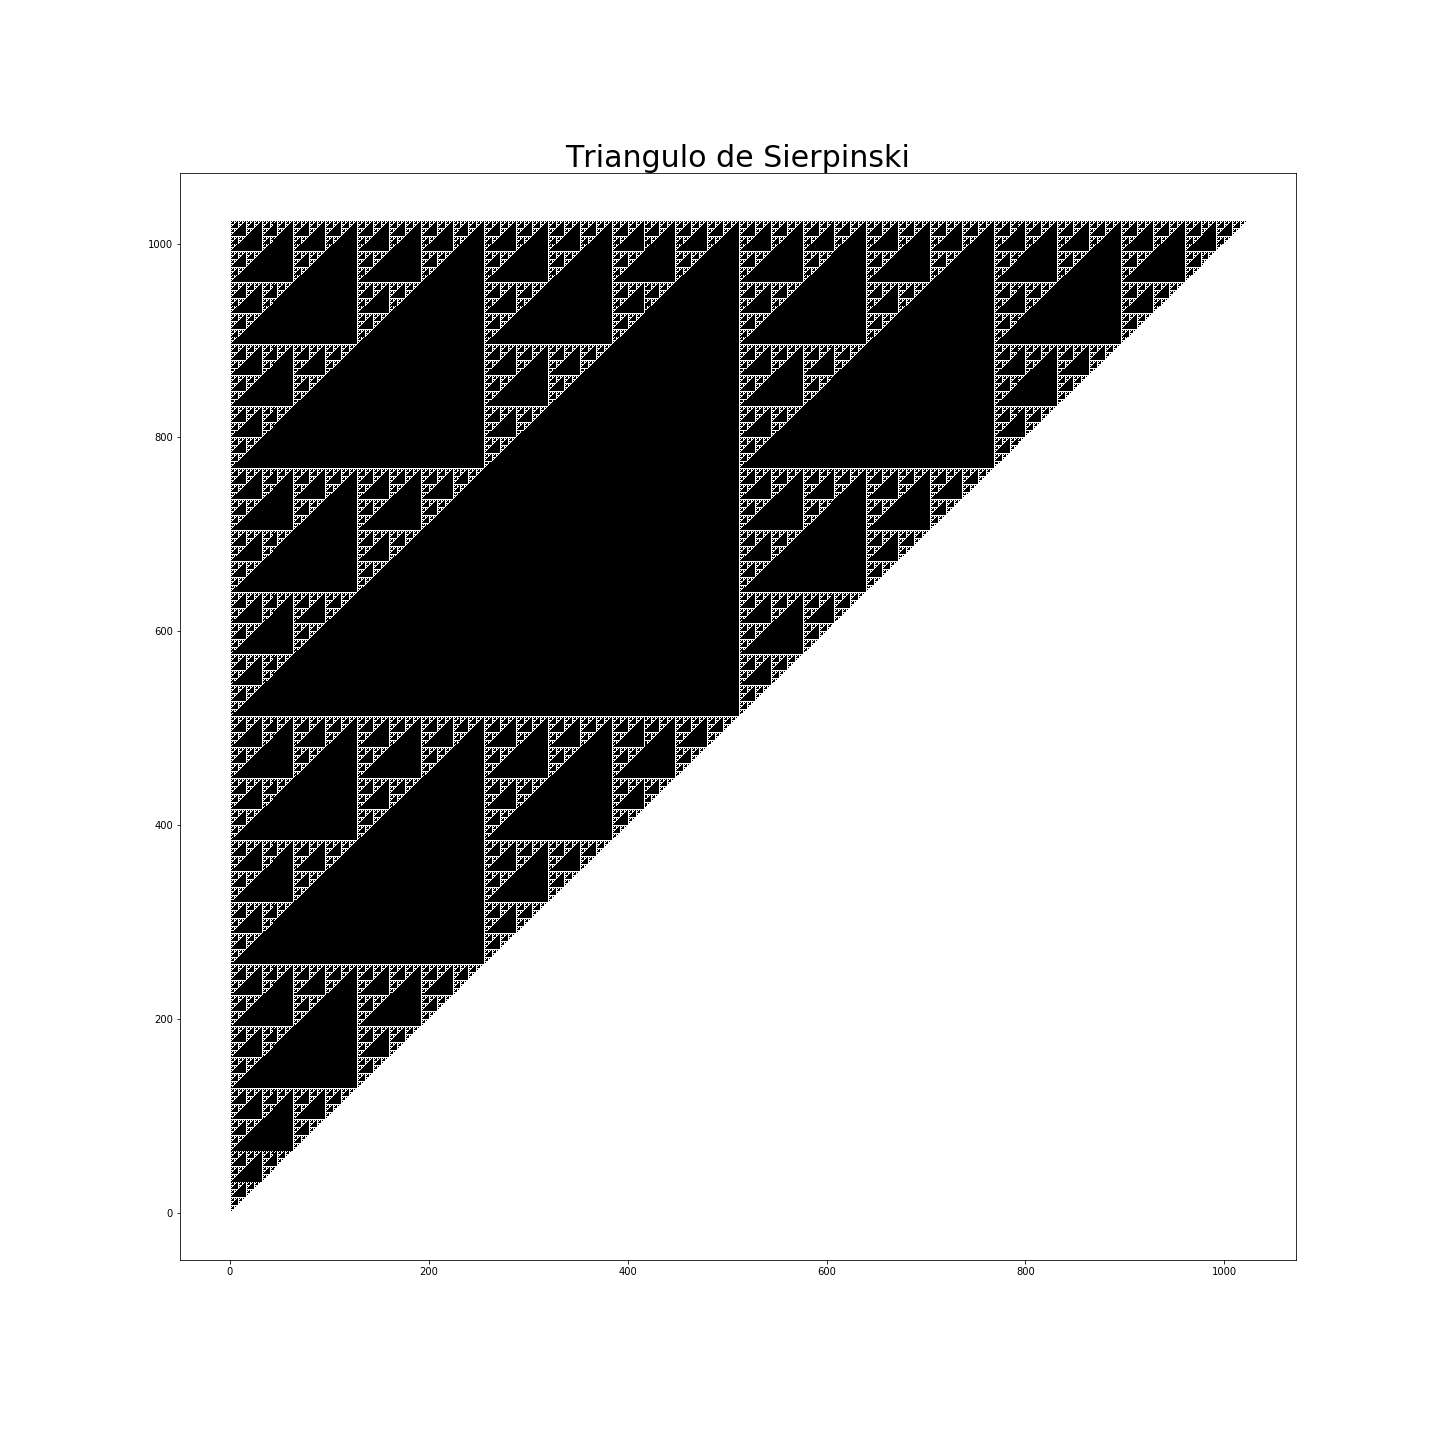
\includegraphics[width=4cm]{triangulo.jpg}
\caption*{\textbf{Figura 6.2} Triángulos de Sierpinski Gasket construido a basel del triangulo de pascal en python}
\label{etiqueta}
\end{figure}

El matemático Benoît Mandelbrot (1924-2011) fue uno de los pioneros que se adentro en la investigación de “la morfología de lo amorfo”. Como el mismo lo menciona en su libro “La geometría fractal de la naturaleza”, los matemáticos huían de lo natural, de las formas que presenta la naturaleza como las ramas de los arboles, las nubes, los rayos, caracoles, entre una infinidad de curiosas formas y patrones que inspiran a un alma apasionada al arte \cite{frac}. Mandelbrot desarrollo una geometría que puede acercarse a describir las formas de la naturaleza. En 1967 publica How Long Is the Coast of Britain? Statistical Self-Similarity and Fractional Dimension \cite{granbre}, donde presenta la paradoja que existe al medir la longitud de la costa de Gran Bretaña (en general de cualquier costa). Esta paradoja consiste en que la longitud de la costa dependerá de la escala de medida que se use. En otras palabras, mientas más grande sea la regla con la que se mide la costa más pequeña será la longitud medida (ver \textbf{figura 6.3}). 

\begin{figure}[H]
\centering
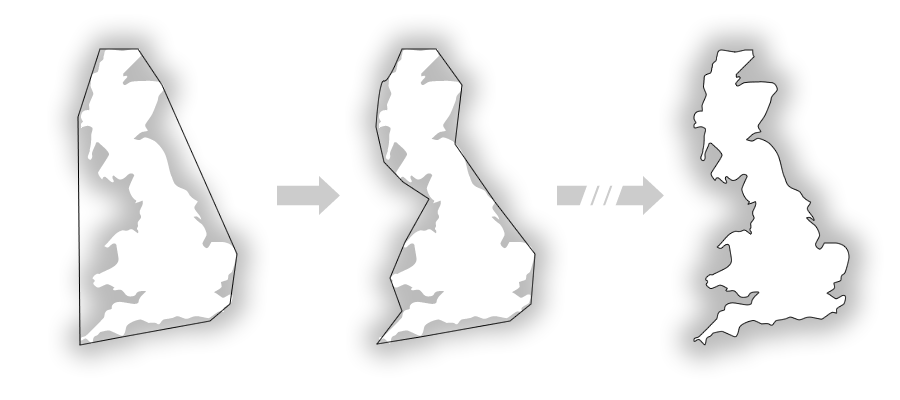
\includegraphics[width=7cm]{england.png}
\caption*{\textbf{Figura 6.3} Análisis gráfico de la paradoja propuesta por Mandelbrot al medir la longitud del perimetro de la costa de gran bretaña \cite{gran}}
\label{etiqueta}
\end{figure}


Este artículo fue de vital importancia  la introducción sobre el concepto de fractal. Ademas, Se tomo el termino latino “fractus” , que usado como verbo significa “romper en pedazos”, para nombrar estas figuras \citar{frac}

Otro ejemplo de fractales son los conjuntos de Julia  que se obtienen al trabajar con funciones complejas. Gaston Julia (1893-1978), matemático francés y uno de los fundadores de la teoría  sistemas dinámicos, trabajo con polinomios en el plano complejo y se dio cuenta que al tener una aplicación iterativa de funciones complejas, $z_{n+1} = f(z_{n})$, se obtenía un conjunto el cual tiene una frontera de longitud infinita, es decir, obtenemos un fractal. Al ser gratificado   éste conjunto se observan de inmediato la forma de un fractal con patrones interesantes. Por ejemplo, con el polinomio en el plano complejo:
\begin{equation*}
f(z) = z^2
\end{equation}
Haremos las iteraciones de tal forma que:
\begin{equation*}
z_{n+1} = z_{n}^2
\end{equation}
Comenzando con el número complejo $w_0 = u + iv = re^{i\theta}$, por lo que las iteraciones quedaran:
\begin{equation}
\begin{split}
&w_0 = re^{i\theta},\\
& w_1 = (w_0)^2 =r^2e^{i2\theta},\\ 
& w_2 = (w_1)^2 =r^4e^{i4\theta}, …,\\
&w_n =(re^{i\theta})^{2^n}
\end{split}
\end{equation}
De aquí podemos deducir el comportamiento de $w$ cuando $n \longrightarrow \infty$. Si $r<1$ cuando  $n \longrightarrow \infty$ $r^{2^n}$ tenderá a cero, y así todos los puntos que se encuentre dentro del circulo unitario en el plano complejo tendían como atractator el origen del plano. Ahora, si $r>1$ cuando  $n \longrightarrow \infty$ los puntos divergen\cite{sd}. A estos puntos los pondremos en un conjunto llamado puntos de escape:
\begin{equation}
\Omega = \{w; |w| \longrightarrow \infty \quad si \quad n \longrightarrow \infty\}
\end{equation}

Y el conjunto de los puntos prisioneros será:
 \begin{equation}
\mho = \{w; w \not\in \Omega\}
\end{equation}

Este grupo contiene a los puntos que su atractor es el origen y los que constituyen la frontera (w tales que $r=1$) los cuales siempre permanecen en ella. A éste de le denomina \textbf{conjunto de Julia} para polinomios $f(z)=z^2$. Estos conjuntos provienen de polinomios de la forma $f(z) = z^2+c$ donde c es un número complejo arbitrario \cite{julia}. Su representación en el plano complejo se puede ver en la \textbf{figura 6.4}. 
\begin{figure}[H]
\centering
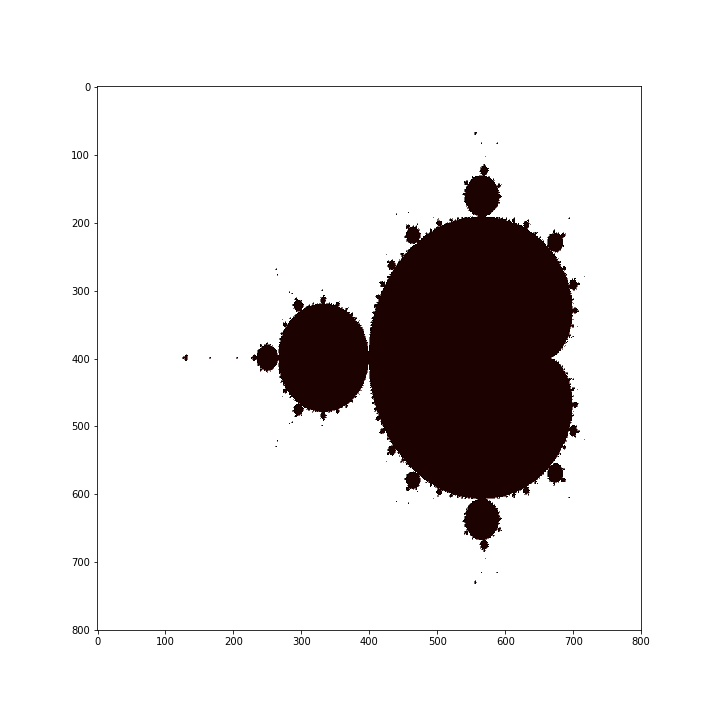
\includegraphics[width=7cm]{fractal.jpg}
\caption*{\textbf{Figura 6.4} Conjunto de Mandelbrot representade en el plano complejo. }
\label{etiqueta}
\end{figure}

Estas figuras y en general el concepto de fractal se a incluido en el arte, no sólo en lo gráfico sino que también en la música. Se an encontrado secuecias en los tiempo y melodias de las obras de Johann Sebastian Bach que pueden concebirse como si fueran fractales musicales. Sin duda alguna, el caos a roto la barrera entre el arte y la ciencia.  

\section{Sistema caótico Mecánico: Modelo de Lotka - Volterra (ecuación de depredador - presa)}

Alfred James Lotka (1880 - 1949) fue un matemático, físico estadounidense quien quien se dedico a la bio-matemática y bio-estadística. En 1925 publico su libro “Elements of Physical Biology” donde presenta un modelo para describir la evolución de una polución de presas junto con la población de sus depredadores. En 1926 Vito Volterra (1860-1940)  publica las mismas ecuaciones ya presentadlas por Lotka en su modelo. Estas ecuaciones son:

\begin{equation}
\begin{split}
\frac{dx}{dt } & = Ax-Bxy \\
\frac{dy}{dt}  & =-Cy+Dxy
\end{split}
\end{equation}

Las cuales tienen una forma parecidas a la del mapeo logístico (ver sección mapeos) debido a la construcción similar de estas. Las ecuaciones conllevan la descripción de la evolución de dos poblaciones de especies distintas: presas $x$ y depredadores $y$. La población de presas, asumiendo que todo el tiempo tienen comida y en ausencia de depredadores, crecerá de manera proporcional a su tamaño, $\dot x = Ax $. Por su parte,  La población de depredadores, asumiendo que no hay presas que casar, disminuida su población de manera proporcional a su tamaño, $\dot y = -Cy$. Al tomar en cuenta las dos especies en el mismo sistema, la población de presas disminuye y la de depredadores aumenta, siendo estos términos proporcionales a la frecuencia de que individuos de cada especie se encuentren, es decir, $-Bxy$ para las presas y $+Dxy$ para los depredadores. De esta forma obtenemos las ecuaciones anteriores con cada parámetro $A, B, C$ y $D$ positivos.

Esta ecuacion puede ser extendida para $N$ especies de a forma:

\begin{equation}
\frac{dx_i}{dt} = r_i x_i \left(1-\sum_{j=1}^N a_{ij} x_j \right)
\end{equation}

siendo $r_i > 0 $ y $a_{ij} > 0$. En el artículo "Chaos in Low-Dimensional Lotka-Volterra Models of Competition" J. A. Vano y colaboradores analizan la aparición del comprtamiento caótico de este sistema cuando se tienen $N = 4$ especies \cite{lv}. El la figura siguinete se muestra el atractor extraño que se forma en este sistema mostrado en el artículo. 

\begin{figure}[H]
\centering
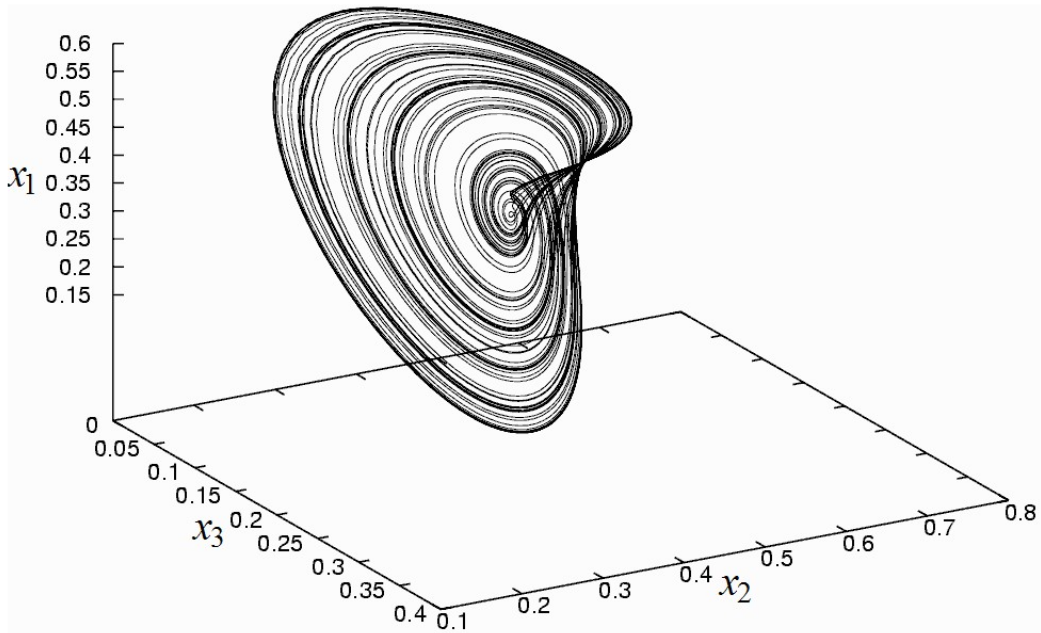
\includegraphics[width=7cm]{presa_atrac.png}
\caption*{\textbf{Figura 7.1} Atractor extreño formado por la coexistencia de 4 especies distintas de presas y depredadores\cite{lv}. }
\label{etiqueta}
\end{figure}

Y el diagrama de bifurcación del sistema, así como su coeficiente de Liapunov se muetra en la \textbf{figura 7.2}. El diagrama de bifurcación muestra el valor de la población $x_1$ despues de cierta cantidad de tiempo variendo un parametro $S$ que multiplica a la matriz de parametros $a_{ij}$ en los elementos fuera de la diagonal.

\begin{figure}[H]
\centering
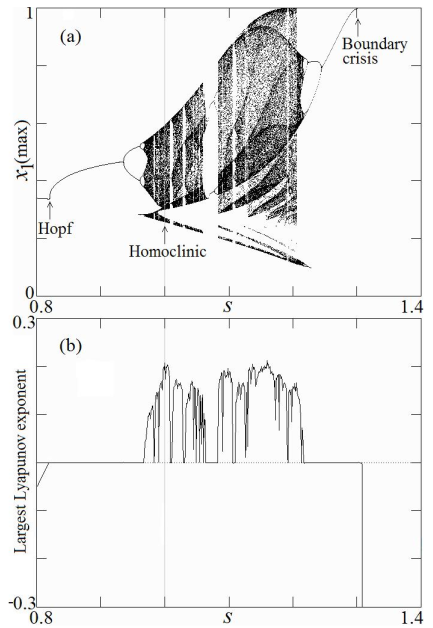
\includegraphics[width=7cm]{presa_bifur.png}
\caption*{\textbf{Figura 7.2} Diagrama de bifurcación y coeficientes de lyapunov del modelo de Lotka - Volterra para $N=4$ especies distintas \cite{lv}. }
\label{etiqueta}
\end{figure}

Donde la matriz $a_{ij}$ viene dada por las ecuaciones:

\begin{equation}
\begin{split}
\frac{dx_1}{dt} &= r_1x_1(1-a_{11}x_1-a_{12}x_2-a_{13}x_3-a_{14}x_4)\\
\frac{dx_2}{dt} &= r_2x_2(1-a_{21}x_1-a_{22}x_2-a_{23}x_3-a_{24}x_4)\\
\frac{dx_3}{dt} &= r_3x_3(1-a_{31}x_1-a_{32}x_2-a_{33}x_3-a_{34}x_4)\\
\frac{dx_4}{dt} &= r_4x_4(1-a_{41}x_1-a_{42}x_2-a_{43}x_3-a_{44}x_4)\\
\end{split}
\end{equation}

y en este caso tenemos:

\begin{equation}
a = 
\begin{bmatrix}
    1    & 1.09 & 1.52  & 0     \\
    0    & 1    & 0.44  & 1.36  \\
    2.33 & 0    & 1     & 0.47  \\
    1.22 & 0.51 & 0.35  & 1
\end{bmatrix}
\end{equation}

y 

\begin{equation}
r = 
\begin{bmatrix}
    1    &  \\
    0.72 &  \\
    1.53 &  \\
    1.27 &  \\
\end{bmatrix}
\end{equation}

\section{Dimeción Fractal}
 
Como se vio en las sección sobre exponente  de Lyapunov, los coeficientes obtenido en un sistema dinámico da información sobre si éste tendrá un comportamiento caótico. Otra método para cuantificar estos aspectos caóticos de los sistemas dinámicos es a travez del aspecto geométrico del atractor formado. Un termino importante en la caracterización de los sistemas es la dimesionalidad en la que se desenvuelve su movimiento. La mínima dimensinalidad en la que se mueve el sistema determina los grados de libertad de éste. 

Los atractores extraños que caracterizan los sistemas caóticos toman forma de fractal los cuales tienen una peculiaridad en sus dimensionalidad ya que es de fraccional. Es decir, si un atractor tiene una dimensión no entera entonces tenemos un atractor extraño. Para obtener la dimensión un fractal primero pensemos en un objeto lineal de tamaño 1 en una dimención. Al reducir su tamaño por un factor $1/R$ en cada dirección, se necesita un número $N(R) = kR^{-D}$ de objetos iguales para cubrir el original (dodne $k$ es una constante de proporcionalidad). por lo tanto se obtiene la siguiente expresión para determinar la dimención \cite{fracwiki} 

\begin{equation}
D =  -\frac{\log N(l)}{\log l} + \frac{\log k}{\log R}
\end{equation}

para un fractal llevamos la divición $1/R$ al infinito y tendremos:
 
\begin{equation}
D = - \lim_{R \rightarrow \infty } \frac{\log N(R)}{\log R} 
\end{equation}  

Dodne $N(R)$ es el número de elementos y $R$ es la longitud lineal de estos. De esta manera encontramos la dimención fraccional de los fractales.

En medicina, como veremos más adelante, se usa la dimención de correlación $D_2$. Esta se calcula con un numero de puntos $N$ al azar sobre una región del espacio euclídio que contenga al fractal. La dimención del fractal será:
\begin{equation}
D_2 = \lim_{R \rightarrow 0,M\rightarrow \infty} \frac{log(g_{R}/M^2)}{\log(R)}
\end{equation}

Dodne $M$ es el número de puntos que caen sobre el fractal y $g_{R}$ es el número de pares de puntos que se encuentran más cercanos.   

\subsection{Neurodinámica}

En la naturaleza podemos encontrar una enorme cantidad de sistemas mecánicos caóticos con propiedades interesantes y bellas formas como hemos visto en los ejemplos de cada tema. Pero uno se los más interesantes y en su mayoría desconocido es la actividad neuronal. El cerebro a sido el objeto de estudio de un sin fin de personas por años y es una maquina tan compleja que el comportamiento caótico debería acompañarlo. Lo sorprendente es que es así, el caos a formado un papel importante en entender la dinámica cerebral y a través de esto se puede plantear la tarea de entender la complejidad de la actividad cerebral con ayuda de teoría del caos.  

\begin{figure}[H]
\centering
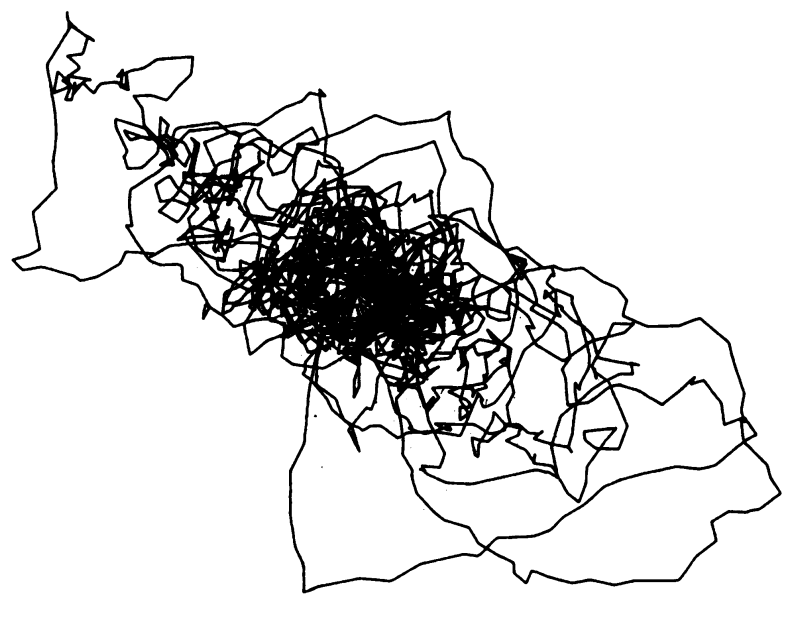
\includegraphics[width=4cm]{atrac_neuro.png}
\caption*{\textbf{Figura 8.1}   Espacio fase del electroencefalograma en la etapa de sueño humano\cite{neuro}. }
\label{etiqueta}
\end{figure}


Agnes Babloyantz y colaboradores de la universidad de Bruselas en 1986 llevaron a cabo estudios de un tipo de epilepsia llamado \textift{petit mal}. Este fonomeno patológico, también llamado crisis de ausencia, presenta convocaciones acompañados de episodios de alteración del estado de conciencia. Por medio de electroencefalogramas tomadas en los episodios de epilepsia de pacientes, A. Babloyantz y A. Destexhe construyen y  muestran la existencia de un atractor consecuencia de la naturaleza determinista de la actividad cerebral (\textbf{figura 8.1})\cite{neuro}. Ademas, los resultados arrojaron un exponente e Lyapunov de $\lambda = 2.9 \pm 0.6$ lo que dio evidencia de ser un atractor extraño junto al valor de la dimensión de correlación $D_2 = 2.05 \pm 0.09$. En la \textbf(tabla 1) se muestra la dimensión de correlación $D_2$ de varios estados del cerebro obtenidas por diversos autores :

Parecen que las dimensiones de correlación están influenciadas por la actividad mental. Vemos que aparecen valores muy bajos para un estado epiléptico. En general en psicopatologías estos valores son mucho más banjos que en sujetos sano. Babloyantz y Destexhe  sugieren que los agentes productores de crisis del tipo “petit mal” tienden a conducir la actividad cerebral hacia un movimiento periódico estable y romper tales estados sería extraordinariamente difícil y sólo posible mediante la dinámica caótica de la actividad cerebral. 

De esta manera, el análisis de la dinámica caótica del sistema cerebral arroja información útil para entender ciertas psicopatologías y así dar una paso mas a su tratamiento efectivo. Así, Las dimensiones de correlación son usadas en medicina por parte de los neurólogos para identificar enfermedades. 

\begin{table}[H]
\begin{tabular}{|c|c|c|}
\hline
\textbf{Autor} & \textbf{Estado/sistema} & \textbf{Resultados} \\ \hline
\begin{tabular}[c]{@{}c@{}}Babloyantz \\ et al.. (1985)\end{tabular} & \begin{tabular}[c]{@{}c@{}}Sueño \\ (estado 2)\\ Sueño\\ (estado 4)\\ Despierto \\ (alfa)\end{tabular} & \begin{tabular}[c]{@{}c@{}}$D_2 = 5.03$\\ $D_2 = 4.0 - 4.4$\\ $D_2 = 6.1$\end{tabular} \\ \hline
\begin{tabular}[c]{@{}c@{}}Rapp et al.. \\ (1986)\end{tabular} & Ojos cerrados & $D_2  = 2.4 - 2.6$ \\ \hline
\begin{tabular}[c]{@{}c@{}}Babloyantz \\ et al.. (1986)\end{tabular} & \begin{tabular}[c]{@{}c@{}}Creutsfeld \\ - Jacob\\ Epilépsia\end{tabular} & \begin{tabular}[c]{@{}c@{}}$D_2 = 3.7 - 5.4$\\ $D_2 = 2.05$\end{tabular} \\ \hline
\end{tabular}

\textbf{Tabla 1}: Dimenciones fractales obtenida por diversos autores csobre distintos estados de electroencefaloframas humanos \cite{tabla} 
\end{table}

\section{Conclusión}

Sin duda alguna, el caos en los sistemas dinámicos es un mundo difícil de dominar. Es una teoría amplia  y compleja que aún tiene mucho que aportar. La tarea de los físicos es encontrar patrones en el comportamiento natural de las cosas y el caos propone un gran desafío para esta tarea pero poder caracterizar el comportamiento caótico de sistemas no lineales nos dan luz verde para un análisis más exhaustivo de los sistemas. Aunque en el texto no pude abarcaron los temas con mayor amplitud lo que he aprendido sobre sistemas dinámicos caoticos me deja satisfecho por ahora pero con con ánimos de seguir aprendiendo su desarrollo. La aplicaciones son amplias, no sólo para física, sino que para todas las ciencias incluyendo a las sociales. La medicina es uno de los usuarios de esta teoría que más me ha sorprendido y es por ello que agregue un poco de ello en el texto. Poder entender una maquina tan compleja como el cerebro y detectar patologías sólo son los primeros pasos, la domesticación del caos nos puede llevar a que éste sea parte del tratamiento y tal vez podamos ir más allá. Tal vez de un poco de miedo deshacerse del determinismo que tanto se presumía en la ciencias como la física pero al fin de cuenta la naturaleza es la que manda. Sólo queda ver a donde nos llevará el caos.

\subsubsection{Bibliografia}\label{sec:bio}

Ilya Prigogine, \emph{Las leyed del caos}, editorial Critica\\

Ricard V. Solé,Susanna C. Manrubia, \emph{Orden y caos ensistemas complejos}, Edicion UPC,Universidad politecnica de Catalunya, (1993)\\

Robert C. Hilborn, \emph{Chaos and Nonlinear Dynamics: "An introduction for scientists and enginners"}, Oxford students edition, (1994)\\

”Sistema dinámico." Wikipedia, La enciclopedia libre. 23 oct 2018, 00:08 UTC. 9 nov 2018, 15:50 $<https://es.wikipedia.org/w/index.php?title=Sistema_din%C3%A1mico&oldid=111469181>.$\\

"Dimensión fractal." Wikipedia, La enciclopedia libre. 27 jul 2018, 10:00 UTC. 12 nov 2018, 05:07 $<https://es.wikipedia.org/w/index.php?title=Dimensi%C3%B3n_fractal&oldid=109558389>.$ \\

Wikipedia contributors, 'Lotka–Volterra equations', Wikipedia, The Free Encyclopedia, 3 October 2018, 00:23 UTC, $<https://en.wikipedia.org/w/index.php?title=Lotka%E2%80%93Volterra_equations&oldid=862227506> [accessed 10 November 2018]$\\

A. BABLOYANTZ
y A. DESTEXHE, \emph{Low-dimensional chaos in an instance of epilepsy}, Faculte des sciences, Universite Libre de Bruxelles (1985)\\

% Bibliografía.
%-----------------------------------------------------------------
\begin{thebibliography}{99}

\bibitem{lig} J. Lighthill, \emph{The recently Recognized Failure  of Predictability in Newtonian Dynamics}, Proceedings of the royal Society, A 407 (1966) pp. 35-50

\bibitem{ilya1} Ilya Prigogine, \emph{Las leyed del caos}, editorial Critica, pp 44

\bibitem{sd} Ricard V. Solé,Susanna C. Manrubia, \emph{Orden y caos ensistemas complejos}, Edicion UPC,Universidad politecnica de Catalunya, (1993) 

\bibitem{Cd94} Robert C. Hilborn, \emph{Chaos and Nonlinear Dynamics: "An introduction for scientists and enginners"}, Oxford students edition, (1994) pg: 19-20

\bibitem{AL} "Atractor de Lorenz.", \emph{Wikipedia, La enciclopedia libre}. 1 oct 2018, 10:57 UTC. 9 nov 2018, 00:00 $<https://es.wikipedia.org/w/index.php?title=Atractor_de_Lorenz&oldid=110981764>. $

\bibitem{ilya2} Ilya Prigogine, \emph{Las leyed del caos}, editorial Critica, pp 46

\bibitem{172} Robert C. Hilborn, \emph{Chaos and Nonlinear Dynamics: "An introduction for scientists and enginners"}, Oxford students edition, (1994) pg: 172

\bibitem{frac} Benoît Mandelbrot, \emph{La geometría fractal de la naturaleza},Tusquets editores,(2013).  

\bibitem{triangulo} Maycon Sedrez, Triângulo de Sierpinski,$ https://www.researchgate.net/figure/Figura-2-Triangulo-de-Sierpinski-Fonte-Do-autor_fig1_280739509$

\bibitem{granbre} Benoît Mandelbrot , (1967). 'How Long Is the Coast of Britain? Statistical Self-Similarity and Fractional Dimension'. en 'Science, New Series, Vol. 156, No. 3775. (May 5, 1967),

\bibitem{gran} AnaliticaWeb, El comportamiento fractal, 23 noviembre, 2017, $https://www.analiticaweb.es/comportamiento-fractal/$

\bibitem{julia} Ricard V. Solé,Susanna C. Manrubia, \emph{Orden y caos ensistemas complejos}, Edicion UPC,Universidad politecnica de Catalunya, (1993) pp 100


\bibitem{lv} J. A. Vano,∗,J. C. Wildenberg, M. B. Anderson, J. K. Noel, y J. C. Sprott, Chaos in Low-Dimensional Lotka-Volterra Models of Competition,  Department of Physics, University of Wisconsin - Madiso, September 24, 2004.

\bibitem{dimen} Robert C. Hilborn, \emph{Chaos and Nonlinear Dynamics: "An introduction for scientists and enginners"}, Oxford students edition, (1994) pg: 394-395

\bibitem{neuro} A. BABLOYANTZ y A. DESTEXHE, \emph{Low-dimensional chaos in an instance of epilepsy}, Faculte des sciences, Universite Libre de Bruxelles (1985)

\bibitem{tabla} Ricard V. Solé,Susanna C. Manrubia, \emph{Orden y caos ensistemas complejos}, Edicion UPC,Universidad politecnica de Catalunya, (1993) pp 499

\bibitem{fracwiki}"Dimensión fractal." Wikipedia, La enciclopedia libre. 27 jul 2018, 10:00 UTC. 12 nov 2018, 05:07 $<https://es.wikipedia.org/w/index.php?title=Dimensi%C3%B3n_fractal&oldid=109558389>.$ 

\end{thebibliography}


\end{document}